%%%%%%%%%%%%%%%%%%%%%%%%%%%%%%%%%%%%%%%%%%%%%%%%%%%%%%%%%%%%%%%%%%%%%%%%%%%%%%%%
%% Plantilla de memoria en LaTeX para la ETSIT - Universidad Rey Juan Carlos
%%
%% Por Gregorio Robles <grex arroba gsyc.urjc.es>
%%     Grupo de Sistemas y Comunicaciones
%%     Escuela T\'ecnica Superior de Ingenieros de Telecomunicaci\'on
%%     Universidad Rey Juan Carlos
%% (muchas ideas tomadas de Internet, colegas del GSyC, antiguos alumnos...
%%  etc. Muchas gracias a todos)
%%
%% La \'ultima versi\'on de esta plantilla est\'a siempre disponible en:
%%     https://github.com/gregoriorobles/plantilla-memoria
%%
%% Para obtener PDF, ejecuta en la shell:
%%   make
%% (las im\'agenes deben ir en PNG o JPG)

%%%%%%%%%%%%%%%%%%%%%%%%%%%%%%%%%%%%%%%%%%%%%%%%%%%%%%%%%%%%%%%%%%%%%%%%%%%%%%%%

\documentclass[a4paper, 12pt]{book}
\usepackage[T1]{fontenc}

\usepackage[a4paper, left=2.5cm, right=2.5cm, top=3cm, bottom=3cm]{geometry}
\usepackage{times}
\usepackage[latin1]{inputenc}
\usepackage[spanish]{babel} % Comenta esta l\'inea si tu memoria es en ingl\'es
\usepackage{url}
\usepackage{nicefrac}
%\usepackage[dvipdfm]{graphicx}
\usepackage{graphicx}
\usepackage{float}  %% H para posicionar figuras
\usepackage[nottoc, notlot, notlof, notindex]{tocbibind} %% Opciones de \'indice
\usepackage{latexsym}  %% Logo LaTeX


\title{Memoria del Proyecto}
\author{Nombre del autor}

\renewcommand{\baselinestretch}{1.5}  %% Interlineado

\begin{document}

\renewcommand{\refname}{Bibliograf\'ia}  %% Renombrando
\renewcommand{\appendixname}{Ap\'endice}

%%%%%%%%%%%%%%%%%%%%%%%%%%%%%%%%%%%%%%%%%%%%%%%%%%%%%%%%%%%%%%%%%%%%%%%%%%%%%%%%
% PORTADA

\begin{titlepage}
\begin{center}
\begin{tabular}[c]{c c}
%\includegraphics[bb=0 0 194 352, scale=0.25]{logo} &

\includegraphics[scale=0.25]{img/logo_vect.png} &
\begin{tabular}[b]{l}
\Huge
\textsf{UNIVERSIDAD} \\
\Huge
\textsf{REY JUAN CARLOS} \\
\end{tabular}
\\
\end{tabular}

\vspace{3cm}

\Large
TITULACI\'oN EN MAY\'uSCULAS

\vspace{0.4cm}

\large
Curso Acad\'emico 2020/2021

\vspace{0.8cm}

Trabajo Fin de Carrera/Grado/M\'aster

\vspace{2.5cm}

\LARGE
T\'iTULO DEL TRABAJO EN MAY\'uSCULAS

\vspace{4cm}

\large
Autor : Nombre del Alumno \\
Tutor : Dr. Gregorio Robles
\end{center}
\end{titlepage}

\newpage
\mbox{}
\thispagestyle{empty} % para que no se numere esta pagina


%%%%%%%%%%%%%%%%%%%%%%%%%%%%%%%%%%%%%%%%%%%%%%%%%%%%%%%%%%%%%%%%%%%%%%%%%%%%%%%%
%%%% Para firmar
\clearpage
\pagenumbering{gobble}
\chapter*{}

\vspace{-4cm}
\begin{center}
\LARGE
\textbf{Proyecto Fin de Carrera}

\vspace{1cm}
\large
FIXME: T\'itulo

\vspace{1cm}
\large
\textbf{Autor :} FIXME \\
\textbf{Tutor :} Dr. Gregorio Robles Mart\'inez

\end{center}

\vspace{1cm}
La defensa del presente Proyecto Fin de Carrera se realiz\'o el d\'ia \qquad$\;\,$ de \qquad\qquad\qquad\qquad \newline de 20XX, siendo calificada por el siguiente tribunal:


\vspace{0.5cm}
\textbf{Presidente:}

\vspace{1.2cm}
\textbf{Secretario:}

\vspace{1.2cm}
\textbf{Vocal:}


\vspace{1.2cm}
y habiendo obtenido la siguiente calificaci\'on:

\vspace{1cm}
\textbf{Calificaci\'on:}


\vspace{1cm}
\begin{flushright}
Fuenlabrada, a \qquad$\;\,$ de \qquad\qquad\qquad\qquad de 20XX
\end{flushright}

%%%%%%%%%%%%%%%%%%%%%%%%%%%%%%%%%%%%%%%%%%%%%%%%%%%%%%%%%%%%%%%%%%%%%%%%%%%%%%%%
%%%% Dedicatoria

\chapter*{}
\pagenumbering{Roman} % para comenzar la numeracion de paginas en numeros romanos
\begin{flushright}
\textit{Dedicado a \\
mi familia / mi abuelo / mi abuela}
\end{flushright}

%%%%%%%%%%%%%%%%%%%%%%%%%%%%%%%%%%%%%%%%%%%%%%%%%%%%%%%%%%%%%%%%%%%%%%%%%%%%%%%%
%%%% Agradecimientos

\chapter*{Agradecimientos}
%\addcontentsline{toc}{chapter}{Agradecimientos} % si queremos que aparezca en el \'indice
\markboth{AGRADECIMIENTOS}{AGRADECIMIENTOS} % encabezado 

Aqu\'i vienen los agradecimientos\ldots Aunque est\'a bien acordarse de la pareja,
no hay que olvidarse de dar las gracias a tu madre, que aunque a veces no lo 
parezca disfrutar\'a tanto de tus logros como t\'u\ldots Adem\'as, la pareja quiz\'as
no sea para siempre, pero tu madre s\'i.

%%%%%%%%%%%%%%%%%%%%%%%%%%%%%%%%%%%%%%%%%%%%%%%%%%%%%%%%%%%%%%%%%%%%%%%%%%%%%%%%
%%%% Resumen

\chapter*{Resumen}
%\addcontentsline{toc}{chapter}{Resumen} % si queremos que aparezca en el \'indice
\markboth{RESUMEN}{RESUMEN} % encabezado

Aqu\'i viene un resumen del proyecto. Ha de constar de tres o cuatro p\'arrafos,
donde se presente de manera clara y concisa de qu\'e va el proyecto. Han
de quedar respondidas las siguientes preguntas:

\begin{itemize}
  \item �De qu\'e va este proyecto? �Cu\'al es su objetivo principal?
  \item �C\'omo se ha realizado? �Qu\'e tecnolog\'ias est\'an involucradas?
  \item �En qu\'e contexto se ha realizado el proyecto? �Es un proyecto
dentro de un marco general?
\end{itemize}

Lo mejor es escribir el resumen al final.

%%%%%%%%%%%%%%%%%%%%%%%%%%%%%%%%%%%%%%%%%%%%%%%%%%%%%%%%%%%%%%%%%%%%%%%%%%%%%%%%
%%%% Resumen en ingl\'es

\chapter*{Summary}
%\addcontentsline{toc}{chapter}{Summary} % si queremos que aparezca en el \'indice
\markboth{SUMMARY}{SUMMARY} % encabezado

Here comes a translation of the ``Resumen'' into English. Please, double check
it for correct grammar and spelling. As it is the translation of the ``Resumen'',
which is supposed to be written at the end, this as well should be filled out
just before submitting.


%%%%%%%%%%%%%%%%%%%%%%%%%%%%%%%%%%%%%%%%%%%%%%%%%%%%%%%%%%%%%%%%%%%%%%%%%%%%%%%%
%%%%%%%%%%%%%%%%%%%%%%%%%%%%%%%%%%%%%%%%%%%%%%%%%%%%%%%%%%%%%%%%%%%%%%%%%%%%%%%%
% \'iNDICES %
%%%%%%%%%%%%%%%%%%%%%%%%%%%%%%%%%%%%%%%%%%%%%%%%%%%%%%%%%%%%%%%%%%%%%%%%%%%%%%%%

% Las buenas noticias es que los \'indices se generan autom\'aticamente.
% Lo \'unico que tienes que hacer es elegir cu\'ales quieren que se generen,
% y comentar/descomentar esa instrucci\'on de LaTeX.

%%%% \'indice de contenidos
\tableofcontents 
%%%% \'indice de figuras
\cleardoublepage
%\addcontentsline{toc}{chapter}{Lista de figuras} % para que aparezca en el indice de contenidos
\listoffigures % indice de figuras
%%%% \'indice de tablas
%\cleardoublepage
%\addcontentsline{toc}{chapter}{Lista de tablas} % para que aparezca en el indice de contenidos
%\listoftables % indice de tablas


%%%%%%%%%%%%%%%%%%%%%%%%%%%%%%%%%%%%%%%%%%%%%%%%%%%%%%%%%%%%%%%%%%%%%%%%%%%%%%%%
%%%%%%%%%%%%%%%%%%%%%%%%%%%%%%%%%%%%%%%%%%%%%%%%%%%%%%%%%%%%%%%%%%%%%%%%%%%%%%%%
% INTRODUCCI\'oN %
%%%%%%%%%%%%%%%%%%%%%%%%%%%%%%%%%%%%%%%%%%%%%%%%%%%%%%%%%%%%%%%%%%%%%%%%%%%%%%%%

\cleardoublepage
\chapter{Introducci\'on}
\label{sec:intro} % etiqueta para poder referenciar luego en el texto con ~\ref{sec:intro}
\pagenumbering{arabic} % para empezar la numeraci\'on de p\'agina con n\'umeros

Los UAV o Drones se han popularizado en los \'ultimos a�os hasta es punto de formar parte de nuestro d\'ia a d\'ia con aplicaciones en muchos ambitos de nuestra vida. 

Si bien se est\'an utilizando ya de forma habitual en sectores como el cine o la ingenier\'ia civil, a\'un se est\'an explorando muchas de las posibles utilidades que estos robots pueden llegar a ofrecer.

El objetivo de este trabajo final es poner en valor y asentar el uso de un tipo de UAV que no est\'a hoy muy representado en el \'ambito civil y que aventaja en varios aspectos al mas popularizado quadrac\'optero, se trata del avi\'on.

\section{Tipos de aeronaves}
\label{sec:tipos_aeronaves}

Las aeronaves son la base sobre las que se asienta la inteligencia que permite que nuestro robot vuele de ah� que convenga dedicar unas l�neas a entender la base de las mismas y en particular las que son objeto de estudio y desarrollo en este PFC los llamados aerodinos.
Existen principalmente 2 tipos de aeronaves si atendemos al modo en que generan su sustentaci\'on con sus alas, de ala fija y las de ala rotatoria.

Dentro de la tipificaci\'on de ala fija tenemos aquellas aeronaves que tienes sus alas fijas al fuselaje.
Seg\'un la definici\'on de la OACI, es un �Aerodino propulsado por motor, que debe su sustentaci\'on en vuelo principalmente a reacciones aerodin\'amicas ejercidas sobre superficies que permanecen fijas en determinadas condiciones de vuelo�
Algunos ejemplos de aeronaves de ala fija son los aeroplanos, planeadores/veleros, aladeltas, parapentes, paramotores y ultraligeros.

Este tipo de aerodinos los conocemos mas com\'unmente como avienes y tienen como principal ventaja de que la carga de aire que necesitan en sus alas puede ser producida de muchas formas distinta (los veleros no tienen ning\'un tipo de propulsi\'on). Esta carga es variable en funci\'on de la superficie alar del mismo y permite por tanto cargas mas grandes que si instal\'asemos el mismo propulsor en un ala rotatoria.
Pongamos como ejemplo el A380 de Airbus, es el avi\'on de pasajeros mas grande del mundo y cuenta con 4 motores que producen un empuje de entre 70.000 y 80.000lbs, unas 32-36 toneladas de empuje cada uno generando por  tanto entre los 4 a m\'aximo rendimiento y optimas condiciones alrededor de 144 toneladas de empuje. Este avi\'on tiene un peso m\'aximo al despegue\footnote{Peso m\'aximo que es capaz de soportar un avi\'on en su maniobra de despegue}\ de entre 560 y 590 toneladas. Tenemos por tanto que necesitamos en este caso \nicefrac{1}{4} del peso total en empuje para despegar este avi\'on.
Si hici\'esemos este mismo ejercicio con un aerodino de ala rotatoria como el Boing AH-64 o Apache con un peso m\'aximo al despegue de 9,5 toneladas necesitar\'iamos que la combinaci\'on que realizan empuje y palas superase esos 9,5 toneladas para siguiera levantar del suelo.
Este tipo de aerodinos son por tanto mas eficientes, r\'apidos, con mayor carga de pago, mayor alcance debido a su menor consumo y mas estables.

Dentro de la tipificaci\'on de ala rotatoria tenemos aquellas aeronaves que producen su sustentaci\'on con el movimiento (rotaci\'on) de sus alas. En este tipo de aeronaves las alas, tambi\'en llamadas "palas" en este tipo de aerodinos, giran en torno a un eje produciendo con este giro la sustentaci\'on necesaria para despegar del suelo.
Algunos ejemplos de este tipo de aeronaves son los helic\'opteros, autogiros, convertibles o los ampliamente conocidos en robotica aerea los quadrac\'opteros.
Este tipo de aerodino tiene como principal ventaja frente a los ala fija en su versatilidad a la hora de realizar las maniobras de despegue y aterrizaje que pueden realizarse de forma vertical (VTOL\footnote{Vertical take off and landing }) adem\'as de la capacidad de realizar vuelo estacionario\footnote{Mantenerse est\'aticamente en un punto elevado} que le hacen imprescindible en escenarios poco accesibles o donde nos es posible aterrizar como el rescate mar\'itimo.


\section{Origenes}
\label{sec:origenes}


Los or\'igenes de la rob\'otica aerea tienen origen militar y su avance ha estado intr\'insecamente ligado a este \'ambito durante todo el siglo XX.

Se consideran el origen de los aviones no tripulados los experimentos llevados a cabo a principios del siglo XX durante la 1� guerra mundial como el "Aerial Target" desarrollado por el capit\'an A. H. Lowpara para su uso como blanco a\'ereo. Si bien eran veh\'iculos no tripulados (Unmaned Aereal Vehicles) no eran aut\'onomos y eran manejados desde tierra a trav\'es de una radio. 
No es hasta el final del siglo XX cuando bajo el escenario de la guerra de Vietnam y ante la creciente perdida de vidas de los pilotos estos veh\'iculos vuelvan de nuevo a ser objeto de desarrollo y se conviertan en veh\'iculos aut\'onomos.

Desde ese momento y hasta nuestros d\'ias se utilizan de forma habitual en el \'ambito militar en misiones de reconocimiento, bombardeos o apoyo sin arriesgar vidas humanas.

A los largo de los primeros a�os de este siglo debido al abaratamiento de los componentes electr\'onicos y a su minituarizaci\'on y potencia, la rob\'otica a\'erea se ha "desmilitarizado" y esta experimentado un enorme crecimiento en el \'ambito de las aplicaciones civiles.

Hoy en d\'ia es com\'un encontrar en cualquier jugueter\'ia quadrac\'opetros radio-pilotados por poco menos de 30 euros y en tiendas especializadas podemos encontrarlos ya con el hardware y software integrados que les permiten seguir una serie de puntos de control y comportarse de forma aut\'onoma por poco mas de 200?.

Por ello se ha popularizado su uso en aplicaciones civiles como:
Fotograf\'ia a\'erea. Para por ejemplo usos topogr\'aficos o educativos e incluso recaudatorios\footnote{El ministerio de hacienda espa�ol tiene varios drones para cotejar los datos catastrales con la vivienda f\'isica}
Cine y televisi\'on. Hoy en d\'ia es raro encontrar una producci\'on que no haya hecho uso de ellos y es que permite la captura de tomas que de otra forma ser\'ian extremadamente complicadas o imposibles o bien factibles pero econ\'omicamente inviables.
Vigilancia y protecci\'on. Las principales fuerzas y cuerpos de seguridad de una gran cantidad de pa\'ises los utilizan.

Se esta experimentando su uso en otros \'ambitos como el log\'istico\footnote{Amazon plantea utilizarlo en algunas entregas}, sanitario o salvamento.

 
\section{Estado del arte}
\label{sec:estado_arte}

En la actualidad el uso de AUV o drones se ha popularizado tanto que es una de las industrias en las que mas ha crecido su inversi\'on, y es que seg\'un la empresa analista especializada en dones Droneii con sede en Hamburgo en un estudio sobre la inversi\'on en el sector\footnote{\url{http://www.droneii.com/drone-investment-trends-2016}} en europa se invirti\'o en en proyectos dom\'esticos en 2016 cerca de 65 millones de d\'olares increment\'andose esta cifra hasta los 314 millones si atendemos al mercado norteamericano.
Estas datos se asientan en un mercado cada vez mas extendido y con una gran proyecci\'on de crecimiento,la publicaci\'on BI Intelligence\footnote{\url{http://www.businessinsider.com/the-drones-report-research-use-cases-regulations-and-issues-2016-4}} espera que las ventas de drones alcancen los 12.000 millones en 2021.

Con su uso ya ampliamente extendido en sectores como el cine, la televisi\'on, fotograf\'ia, agropecuario, educativo, forestal, ingenier\'ia civil y presencia en sectores como el sanitario, salvamento o seguridad y protecci\'on el nicho de mercado de los UAV esta lejos de su cima y se investigan dia a dia nuevos usos en sectores como la log\'istica.

Dentro del laboratorio de rob\'otica de la Universidad Rey Juan Carlos cabe destacar los trabajos realizados para profundizar investigar y experimentar con ellos.
Trabajos como el de Alberto Mart\'inez Florido quien desarrollo un driver para poder utilizar desde jderobot el ar-drone comercial, desarrollado por la empresa francesa parrot, y el software de control UAV Viewer. Y mas adelante Daniel Yague que realiz\'o un driver para utilizar el ar-drone de forma simulada en gazebo.
O los trabajos de Jorge Cano quien construyo propio su drone utilizando como base un quadrac\'optero y dando soporte a jderobot de muchas de las intruciones de MAVLink.
Son destacables tambi�n los trabajos que se est�n llevando a cabo por Diego Jimenez adaptando el interfaz SoloDrone de la empresa 3DR\footnote{Empresa norteamericana con sede en California especializada en rob�tica a�rea. Se sit�a en 2017 como la 3� empresa del sector} o Jorge Vela quien se encuentra desarrollando como realizar la maniobra de aterrizaje de forma autom�tica.

\section{Objetivos}
\label{sec:objetivos}

Los objetivos de este PFC son arrojar luz sobre el uso de drones de ala fija poniendo en valor �stos en situaciones donde la carga de pago, la autonom�a, velocidad o consumo desaconsejan el uso de los mas extendidos quadrac\'opteros.

Para �sto hemos adaptado un avi�n de radio-control comercial a�adi�ndole toda la avi�nica necesaria para que puede operar como drone. Hemos desarrollado un driver para jderobot del interfaz MAVLink que nos permite recoger actitud, velocidades lineales y angulares, altura, posici�n y otros par�metros como la bater�a restante. Nos permite tambi�n la actuaci�n con el seguimiento de misiones que no s�lo incluyen el paso por ciertos puntos de control o waypoints sino que tambi�n soporta las maniobras de despegue y aterrizaje en drones de ala fija.
Hemos desarrollado tambi�n un software de control que da soporte a este tipo de actuaci�n de mas alto nivel, las misiones.

\section{Estructura de la memoria}
\label{sec:estructura}

En esta secci\'on se deber\'ia introducir la esctura de la memoria. As\'i:

\begin{itemize}
  \item En el primer cap\'itulo se hace una intro al proyecto.
  
  \item En el cap\'itulo~\ref{chap:objetivos} se muestran los objetivos del proyecto.
  
  \item A continuaci\'on se presenta el estado del arte.
  
  \item \ldots
\end{itemize}



%%%%%%%%%%%%%%%%%%%%%%%%%%%%%%%%%%%%%%%%%%%%%%%%%%%%%%%%%%%%%%%%%%%%%%%%%%%%%%%%
%%%%%%%%%%%%%%%%%%%%%%%%%%%%%%%%%%%%%%%%%%%%%%%%%%%%%%%%%%%%%%%%%%%%%%%%%%%%%%%%
% OBJETIVOS %
%%%%%%%%%%%%%%%%%%%%%%%%%%%%%%%%%%%%%%%%%%%%%%%%%%%%%%%%%%%%%%%%%%%%%%%%%%%%%%%%

\cleardoublepage
\chapter{Objetivos}
\label{chap:objetivos}

\section{Objetivo general}
label{sec:objetivo-general}


\section{Objetivos espec\'ificos}
label{sec:objetivos-especificos}


\section{Planificaci\'on temporal}
label{sec:planificacion-temporal}



%%%%%%%%%%%%%%%%%%%%%%%%%%%%%%%%%%%%%%%%%%%%%%%%%%%%%%%%%%%%%%%%%%%%%%%%%%%%%%%%
%%%%%%%%%%%%%%%%%%%%%%%%%%%%%%%%%%%%%%%%%%%%%%%%%%%%%%%%%%%%%%%%%%%%%%%%%%%%%%%%
% ESTADO DEL ARTE %
%%%%%%%%%%%%%%%%%%%%%%%%%%%%%%%%%%%%%%%%%%%%%%%%%%%%%%%%%%%%%%%%%%%%%%%%%%%%%%%%

\cleardoublepage
\chapter{Estado del arte}

Descripci\'on de las tecnolog\'ias que utilizas en tu trabajo. Con dos o tres p\'arrafos por cada tecnolog\'ia, vale.


Puedes citar libros, como el de Bonabeau et al. sobre procesos estigm\'ergicos~\cite{bonabeau:_swarm}. % Nota que el ~ a�ade un espacio en blanco, pero no deja que exista un salto de l\'inea. Imprescindible ponerlo para las citas.

Tambi\'en existe la posibilidad de poner notas al pie de p\'agina, por ejemplo, 
una para indicarte que visite la p\'agina de 
LibreSoft\footnote{\url{http://www.libresoft.es}}.

\section{Secci\'on 1} 
\label{sec:seccion1}



%%%%%%%%%%%%%%%%%%%%%%%%%%%%%%%%%%%%%%%%%%%%%%%%%%%%%%%%%%%%%%%%%%%%%%%%%%%%%%%%
%%%%%%%%%%%%%%%%%%%%%%%%%%%%%%%%%%%%%%%%%%%%%%%%%%%%%%%%%%%%%%%%%%%%%%%%%%%%%%%%
% DISE�O E IMPLEMENTACI\'oN %
%%%%%%%%%%%%%%%%%%%%%%%%%%%%%%%%%%%%%%%%%%%%%%%%%%%%%%%%%%%%%%%%%%%%%%%%%%%%%%%%

\cleardoublepage
\chapter{Dise�o e implementaci\'on}

\section{Arquitectura general} 
\label{sec:arquitectura}

figura~\ref{fig:arquitectura}.

\begin{figure}
  \centering
  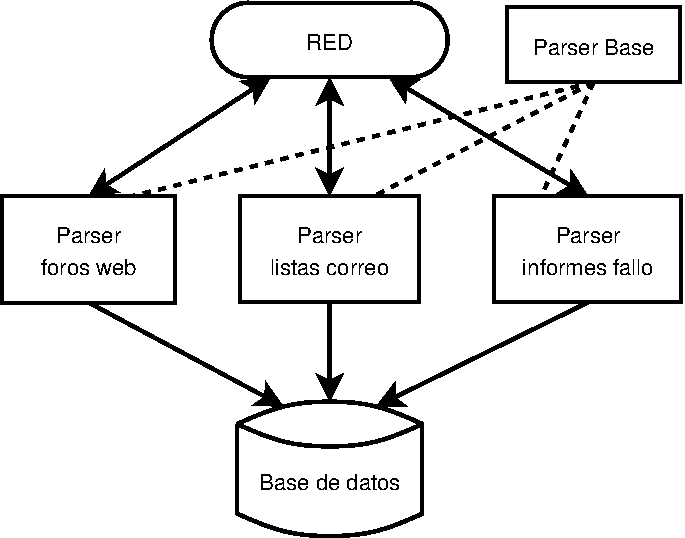
\includegraphics[width=9cm, keepaspectratio]{img/arquitectura}
  \caption{Estructura del parser b\'asico}
  \label{fig:arquitectura}
\end{figure}


%%%%%%%%%%%%%%%%%%%%%%%%%%%%%%%%%%%%%%%%%%%%%%%%%%%%%%%%%%%%%%%%%%%%%%%%%%%%%%%%
%%%%%%%%%%%%%%%%%%%%%%%%%%%%%%%%%%%%%%%%%%%%%%%%%%%%%%%%%%%%%%%%%%%%%%%%%%%%%%%%
% RESULTADOS %
%%%%%%%%%%%%%%%%%%%%%%%%%%%%%%%%%%%%%%%%%%%%%%%%%%%%%%%%%%%%%%%%%%%%%%%%%%%%%%%%

\cleardoublepage
\chapter{Resultados}




%%%%%%%%%%%%%%%%%%%%%%%%%%%%%%%%%%%%%%%%%%%%%%%%%%%%%%%%%%%%%%%%%%%%%%%%%%%%%%%%
%%%%%%%%%%%%%%%%%%%%%%%%%%%%%%%%%%%%%%%%%%%%%%%%%%%%%%%%%%%%%%%%%%%%%%%%%%%%%%%%
% CONCLUSIONES %
%%%%%%%%%%%%%%%%%%%%%%%%%%%%%%%%%%%%%%%%%%%%%%%%%%%%%%%%%%%%%%%%%%%%%%%%%%%%%%%%

\cleardoublepage
\chapter{Conclusiones}
\label{chap:conclusiones}


\section{Consecuci\'on de objetivos}
\label{sec:consecucion-objetivos}

Esta secci\'on es la secci\'on espejo de las dos primeras del cap\'itulo de objetivos,
donde se planteaba el objetivo general y se elaboraban los espec\'ificos.

Es aqu\'i donde hay que debatir qu\'e se ha conseguido y qu\'e no. Cuando algo no
se ha conseguido, se ha de justificar, en t\'erminos de qu\'e problemas se han
encontrado y qu\'e medidas se han tomado para mitigar esos problemas.


\section{Aplicaci\'on de lo aprendido}
\label{sec:aplicacion}

Aqu\'i viene lo que has aprendido durante el Grado/M\'aster y que has aplicado
en el TFG/TFM. Una buena idea es poner las asignaturas m\'as relacionadas y
comentar en un p\'arrafo los conocimientos y habilidades puestos en pr\'actica.

\begin{enumerate}
  \item a
  \item b
\end{enumerate}


\section{Lecciones aprendidas}
\label{sec:lecciones_aprendidas}

Aqu\'i viene lo que has aprendido en el Trabajo Fin de Grado/M\'aster.

\begin{enumerate}
  \item a
  \item b
\end{enumerate}


\section{Trabajos futuros}
\label{sec:trabajos_futuros}

Ning\'un software se termina, as\'i que aqu\'i vienen ideas y funcionalidades
que estar\'ia bien tener implementadas en el futuro.

Es un apartado que sirve para dar ideas de cara a futuros TFGs/TFMs.


\section{Valoraci\'on personal}
\label{sec:valoracion}

Finalmente (y de manera opcional), hay gente que se anima a dar su punto de
vista sobre el proyecto, lo que ha aprendido, lo que le gustar\'ia haber aprendido,
las tecnolog\'ias utilizadas y dem\'as.



%%%%%%%%%%%%%%%%%%%%%%%%%%%%%%%%%%%%%%%%%%%%%%%%%%%%%%%%%%%%%%%%%%%%%%%%%%%%%%%%
%%%%%%%%%%%%%%%%%%%%%%%%%%%%%%%%%%%%%%%%%%%%%%%%%%%%%%%%%%%%%%%%%%%%%%%%%%%%%%%%
% AP\'eNDICE(S) %
%%%%%%%%%%%%%%%%%%%%%%%%%%%%%%%%%%%%%%%%%%%%%%%%%%%%%%%%%%%%%%%%%%%%%%%%%%%%%%%%

\cleardoublepage
\appendix
\chapter{Manual de usuario}
\label{app:manual}


%%%%%%%%%%%%%%%%%%%%%%%%%%%%%%%%%%%%%%%%%%%%%%%%%%%%%%%%%%%%%%%%%%%%%%%%%%%%%%%%
%%%%%%%%%%%%%%%%%%%%%%%%%%%%%%%%%%%%%%%%%%%%%%%%%%%%%%%%%%%%%%%%%%%%%%%%%%%%%%%%
% BIBLIOGRAFIA %
%%%%%%%%%%%%%%%%%%%%%%%%%%%%%%%%%%%%%%%%%%%%%%%%%%%%%%%%%%%%%%%%%%%%%%%%%%%%%%%%

\cleardoublepage

% Las siguientes dos instrucciones es todo lo que necesitas
% para incluir las citas en la memoria
\bibliographystyle{abbrv}
\bibliography{memoria}  % memoria.bib es el nombre del fichero que contiene
% las referencias bibliogr\'aficas. Abre ese fichero y mira el formato que tiene,
% que se conoce como BibTeX. Hay muchos sitios que exportan referencias en
% formato BibTeX. Prueba a buscar en http://scholar.google.com por referencias
% y ver\'as que lo puedes hacer de manera sencilla.
% M\'as informaci\'on: 
% http://texblog.org/2014/04/22/using-google-scholar-to-download-bibtex-citations/

\end{document}
